\section{Localisation}
Mobile robots navigating in accordance to a map, need localisation.
There are various localisation methods and sensors for mobile robots.
This section describes how a localisation method was implemented % on a 'Nexus Robot'
with data from the robot's encoders and its laser range scanner.
Due to time constraints, the method was implemented as an offline program
on a PC, using data gathered by a Nexus Robot, instead of as an online program
running on the Nexus Robot as it moved.
\subsection{Method}
For the localisation part of the project it was chosen to compare two different approaches:

\begin{itemize}
	\item Position estimate based on odometry (wheel encoders).
	\item Position estimate based on line features extracted from the laser range scanner. 
\end{itemize}

Both of these approaches rely on a known starting location.
The second also needs knowledge of the environment
 - it must  compare the extracted features with probable features from the map
(based on last know location of the robot). 


The mobile robot used is a Nexus Robot - 2WD mobile robot kit 10004,
fitted with a laser range scanner of type Hokuyo URG-04LX-LG. 

\begin{figure}[ht]
\centering
  \begin{subfigure}[t]{0.3\textwidth}
    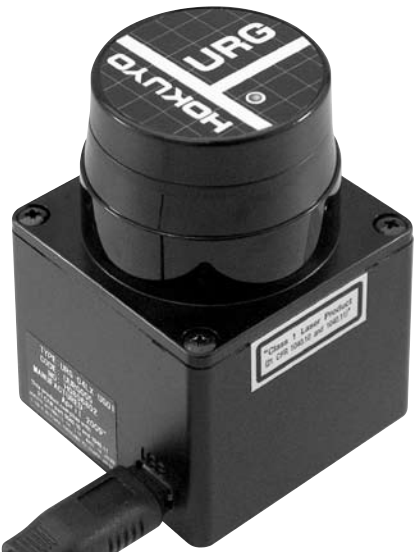
\includegraphics[width = \textwidth]{graphics/hokuyo_laserrange}
    \caption{Hokuyo URG-04LX-LG laser range scanner.}
    \label{laserrange}
  \end{subfigure}
  \begin{subfigure}[t]{0.4\textwidth}
    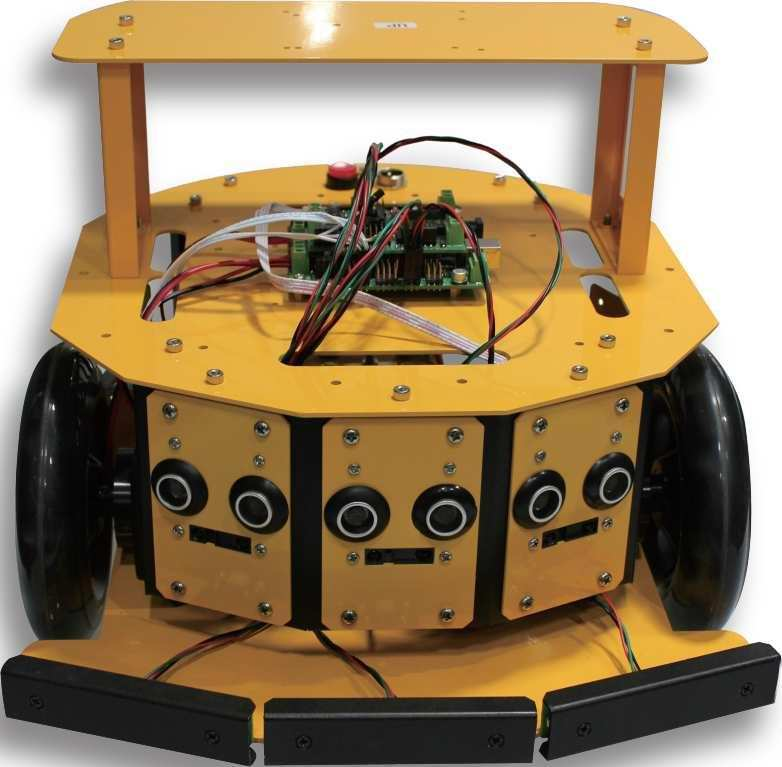
\includegraphics[width = \textwidth]{graphics/nexus_robot}
    \caption{Nexus Robot - 2WD mobile robot kit 10004.}
    \label{laserrange}
  \end{subfigure}
\end{figure}

\subsubsection{Gathering data using UMBmark}
The performance of the localisation technique was measured using UMBmark. 
The position before and after following a preprogrammed path through a 1 x 1 [m] square %5 times
was compared for the different localisation techniques.
%The planned path is shown in figure 
%\todo[inline, author=Michael]{I need picture of it here..}
While testing, the robot was not given any feedback from the sensors.
After each $90 \deg$ turn, the robot stopped and its position on the test track was measured for reference.  
Sensor readings from both the encoders and the laser range scanner were gathered and saved for further offline processing. 
This means that 3 different measurements of the position were gathered: 
\begin{itemize}
	\item Reference position (measured with tape)
	\item Position based on encoder feedback. 
	\item Position based on feature extraction using the laser range scanner. 
\end{itemize}

\subsubsection{Position based on odometry}
%\todo[inline, author=Michael]{Based on (or ripped off :P ) sec. 5.2.4 from our lovely friend, siegwart.}
The position/state $Q$ of the robot is represented by the vector: 
\begin{equation}
  Q_r = 
  \begin{bmatrix}
    x_r \\
    y_r \\
    \alpha_r
  \end{bmatrix}
\end{equation}
The robots position is estimated from the previous position, plus the movement in the last time period $\Delta t$.
The change in position $\Delta Q_r$ from each timestep is added to the position.
This can be written as 
\begin{equation}
  Q_r\textrm' = Q_r + \Delta Q_r
\end{equation}
The feedback from the robot is given as the movement of each wheel in millimetres.
$\Delta Q_r$ can be found from the following equations: 
\begin{eqnarray}
	\Delta x_r &=& \Delta s \cos \left(\alpha_r + \frac{\Delta \alpha_r}{2}\right) \\
	\Delta y_r &=& \Delta s \sin \left(\alpha_r + \frac{\Delta \alpha_r}{2}\right) \\
	\Delta \alpha_r &=& \frac{\Delta s_r + \Delta s_l}{b} \\
	\Delta s &=& \frac{\Delta s_r + \Delta s_l}{2} \\
\end{eqnarray}
Where $\Delta s_r and \Delta s_l$ are the distances traveled by the right and the left wheels
and $b$ is the distance between the robots two wheels. Adding this together, the equation for the updated position is: 
\begin{equation}
  Q_r\textrm' = 
  \begin{bmatrix}
    x_r \\
    y_r \\
    \alpha_r
  \end{bmatrix}
  +
  \begin{bmatrix}
    \Delta s \cos \left(\alpha_r + \frac{\Delta \alpha_r}{2}\right) \\
    \Delta s \sin \left(\alpha_r + \frac{\Delta \alpha_r}{2}\right) \\
    \frac{\Delta s_r + \Delta s_l}{b}
  \end{bmatrix}
\end{equation}
%\todo[inline, author=Michael]{Maybe add an interfacing of scanner subsubsection here?}
%\todo[inline, author=Michael]{And so he wrote a section :P}
\subsubsection{Getting data from the laser range scanner}
The Hokuyo laser scanner measures distance to the nearest obstacles in a $240 \degree$ range. The angular resolution is $0.352 \degree$ which gives 681 data points for each scan. The scanning rate is 10 Hz.

The laser range scanner communicates with the computer using Serial over USB. The serial communication uses the SCIP 2.0 serial protocol. 
A basic application for gathering data from the laser range was written
in C++\footnote{The program is called "hokuyo\_laserrange" in the included "code" directory}.
The program gathers and decodes the data received, and saves it as a CSV file.
The program stops the laser range scanner when the UMBmark test is terminated.

%%%%%%%%%%%
% \input{./content/localisation/ransac}
%%%%%%%%%%%%

\subsubsection{Position based on features from laser range scanner}
The state of the robot is in polar coordinates represented  as 
$$Q_r = \begin{pmatrix}
R_r\\
\theta_r\\
\alpha_r
\end{pmatrix}$$ 
and in cartesian coordinates as 
$$Q_r = \begin{pmatrix}
x_r\\
y_r\\
\alpha_r
\end{pmatrix}$$

When the localisation program starts, it has a map of the room the robot is in.
The map consists four walls, each represented as 
$$wall_n = \begin{pmatrix}
R_n\\
\theta_n
\end{pmatrix}
$$

The initial position of the robot is also known on startup.

The localisation algorithm is illustrated as a flowchart in figure \ref{fig:localisation}.

\paragraph*{Mapping}
The found lines are all represented in the robot's coordinate system, relative to the robot position and orientation.
These lines are mapped into the global map, using the last known robot state. Using 
the last known state of the robot to map the lines will give some mapping-error.
The found lines are then compared to the map. If a found line matches a line 
in the map, within a certain threshold, it is concluded, that they are in 
reality the same line and that the difference is due to the mapping error.

\paragraph*{Updating robot state}
There are several scenarios of what the program will do after the matching of lines,
depending on the lines that have been matched.
The philosophy of the algorithm is that the lines should be used as much as possible,
to determine the robot state.

If no lines have been matched, the robot state remains the same, and is not updated.

If only one line has been matched, the robot orientation \(\alpha_r\) will be updated
so that the found line aligns with the known line in the global map.
The same strategy is used if there are several matched lines, and the new \(\alpha_r\) is
found by averaging the individual orientations.

The robots position will also be updated using as much line information as possible.
If one line has been found, the robots new position is constrained to this line,
and is simply calculated as the nearest point on the line, from the last position.
If two parallel lines have been found, the same strategy is used, and the new position is the average of the two results.
Finding the constraining lines is a matter of moving the global lines towards the origin
by the distances from the robot to the walls.

If two intersecting lines have been matched (and a corner found), the robots position is constrained to
an intersection between two lines. Again, finding the intersection is a matter of moving the global
lines towards the origin by the distance from the robot to the walls,
and then finding the intersection between the two lines.
If more than two intersecting lines are matched, the same strategy is used and the new position
is calculated as the average of all the found positions.

Thus, as long as at least one line is matched, the robot state is updated.
The update correctness should improve with the number of lines matched,
especially if the lines are not parallel.

The weakness of the algorithm lies in missed data points, or data points with no lines detected by RanSaC.
The further the robot actually moves from the last updated position, the harder it is to match the line
feature to the global map, and eventually the lines would be matched incorrectly.

\begin{figure}
  \includestandalone{./content/localisation/flowchart}
  \caption{The localisation method, purely based on data from laser range scanner.}
  \label{fig:localisation}
\end{figure}

